\documentclass{report}

\usepackage[utf8]{inputenc}  
\usepackage[T1]{fontenc}    
\usepackage[french]{babel}
\usepackage{fullpage}
\usepackage{graphicx}
\usepackage{pst-all}

\title{Programmation Graphique Haute Performance\\Simulateur de descente\\Master Informatique Image, son vidéo\\Université Bordeaux 1}
\author{Alexandre Dupouy\\Michaël Morgan\\Arthur Van Poucke}
\date{\today}

\begin{document}
 
\maketitle

\newpage

\tableofcontents

\newpage

\subsubsection*{Introduction}

Dans le cadre de l'unité d'enseignement programmation graphique haute performance il nous est demandé de réaliser un simulateur de descente. Ce travail nous permettra de mettre en œuvres les compétences et les savoirs acquis lors du cours et des différents TD.


Le résultat obtenu devra ressembler au jeu Tuxracer où un avatar glisse sur une pente en évitant les obstacles du terrain tout en respectant les lois de la physique.


Ce projet est composé de plusieurs étapes, d'abord la mise en place du terrain, de l'avatar, et de l'environnement.


Pour finir, nous devrons mettre en place des jeux d'ombres et de lumière sur la scène. 

\chapter{Mise en place du terrain, de l'avatar et de la caméra}

\section{Le terrain}

\subsection*{La génération}
La génération de notre terrain se fait dans un programme séparé du projet en lui-même. Nous présenterons la méthode de génération, ce qui nous a motivé à procéder ainsi, en précisant les avantages et inconvénients de notre implémentation et enfin, les améliorations que nous pourrons apporter par la suite à notre algorithme de génération de terrain.

Nous générons le terrain à partir d’une image en niveaux de gris. Les dimensions du terrain sont les dimensions de l’image qui a servi à le générer (une image de 512 x 512 pixels donnera un terrain de 512 x 512 sommets par exemple). Le niveau de gris de chaque pixel nous donne l’altitude du sommet qui à les mêmes coordonnées. Un pixel noir permet ainsi d’avoir une altitude de 0, alors qu’un pixel blanc nous donnera une altitude de -255. Avec un dégradé de noir vers blanc (de gauche à droite dans l’image), nous générons ainsi une pente sur laquelle notre avatar pourra se déplacer librement. Les ratios utilisés seront amenés à changer dans le développement futur du projet, pour avoir un terrain plus lisse, moins “accidenté”.

Afin de faciliter la création du terrain, nous avons implémenté une classe PgmReader, qui permet de lire une image au format pgm (Portable Grayscale Map). Cette classe stocke dans un buffer toutes les données contenues dans l’image, c’est-à-dire sa largeur, hauteur et les niveaux de gris de tous les pixels.

\subsection*{Particularité de l'implémentation}
Notre implémentation nous permet de générer en moins de 0.5 seconde (cela dépend des caractéristiques de l’ordinateur qui lance le programme) un terrain de 1000 x 400, soit 40000 sommets et 398601 faces, dans un fichier au format off, permettant ainsi un partage facile des terrains générés par les utilisateurs. Cette implémentation nous a permis aussi de pouvoir réutiliser directement le code sur lequel nous avons travaillé durant les séances de TD, réduisant ainsi le temps de développement de cette partie du projet.

\subsection*{Améliorations}
Quelques améliorations sont réalisables sur notre algorithme. Nous pourrons modifier les ratios qui déterminent la largeur, longueur et hauteur de notre terrain, ainsi que permettre d’utiliser directement les images générées avec The Gimp. En effet, The Gimp ajoute une ligne de commentaire dans ses fichiers, et nous ne gérons pour le moment pas cette ligne-ci. Il faut donc, pour que le programme fonctionne, supprimer manuellement les commentaires des fichiers utilisés pour générer le terrain avec un éditeur de texte quelconque.

Cependant, notre manière de générer le terrain ne nous permettra probablement pas d’implémenter l’amélioration consistant à réduire le nombre de sommets/faces à afficher et à ajouter du brouillard, afin d’augmenter la performance du programme.

\section{L'avatar}

\subsection*{Chargement du modèle}
Le chargement du modèle se fait à l'aide de la classe Mesh que nous avons déjà utilisé en TD. La réutilisation de cette classe, déjà bien conçue, nous a permis de réduire notre temps de développement et de pouvoir penser aux autres problèmes du sujet.

\subsection*{Déplacement}
Après avoir placé le modèle sur le terrain et fait en sorte qu'il ne dépasse pas les limites du terrain nous avons simplement stockés à l'aide d'un vecteur les déplacements de l'avatar demandés par l'utilisateur. Il nous suffit d'appliquer ces changements au niveau des shaders pour que le résultat s'observe à l'écran.\\


L'avatar doit aussi suivre le relief du terrain, pour ceci un calcul des normales de chaque point du terrain est nécessaire. C'est dans la classe Mesh que ces calculs sont effectués, nous avons aussi implémenté une fonction qui permet à partir de deux coordonnées x et y de retrouver l'altitude du terrain et la normale en ces coordonnées x et y. L'altitude nous permet de positionner à la bonne hauteur notre avatar. La normale quant à elle, nous permet de d'orienter l'avatar et qu'il ne rentre pas dans le terrain. Pour cela, on effectue un produit vectoriel afin de récupérer le sinus de l'angle formé à partir de l'objet et du terrain pour effectuer la rotation nécessaire sur l'avatar.\\


Il est possible d'améliorer la gestion de l'altitude de l'avatar, en faisant une interpolation des altitudes de tous les sommets de la face sur laquelle l'avatar se trouve.

\section{La caméra}
La camera est toujours placée derrière l'avatar et au dessus de celui-ci. Grâce au même procédé que pour trouver l'altitude de notre avatar sur le terrain, nous pouvons faire en sorte que la caméra ne passe jamais sous le terrain. Le point de visé de la caméra est le centre de notre avatar. Ainsi, sauf dans le cas d'une diminution de pente abrupte (la dérivée de la pente passant de 0 à -50 par exemple), l'avatar est toujours visible par l'utilisateur.\\

Nous pouvons également zoomer/dezoomer sur l'avatar à l'aide des touches +/- et passer de la vue fil de fer/plaine à l'aide des touches 1 et 2.
	
\section{Texturisation}
Des textures ont été appliquées sur le terrain et l'avatar. Cependant un soucis reste sur la texture de l'avatar : lors d'un mouvement, la texture se déplace sur celui-ci.
	 
\section{Éclairage}	
La lumière portée sur la scène est identique à celle du TD : nous avons choisi de conserver le modèle Blinn-Phong.
Nous avons de plus ajouté un éclairage ambiant pour éviter de trop grosses zones d'ombre.

\chapter{Aperçus du programme}

\begin{figure}[hbtp]
\caption{Lancement du jeu}
\centering
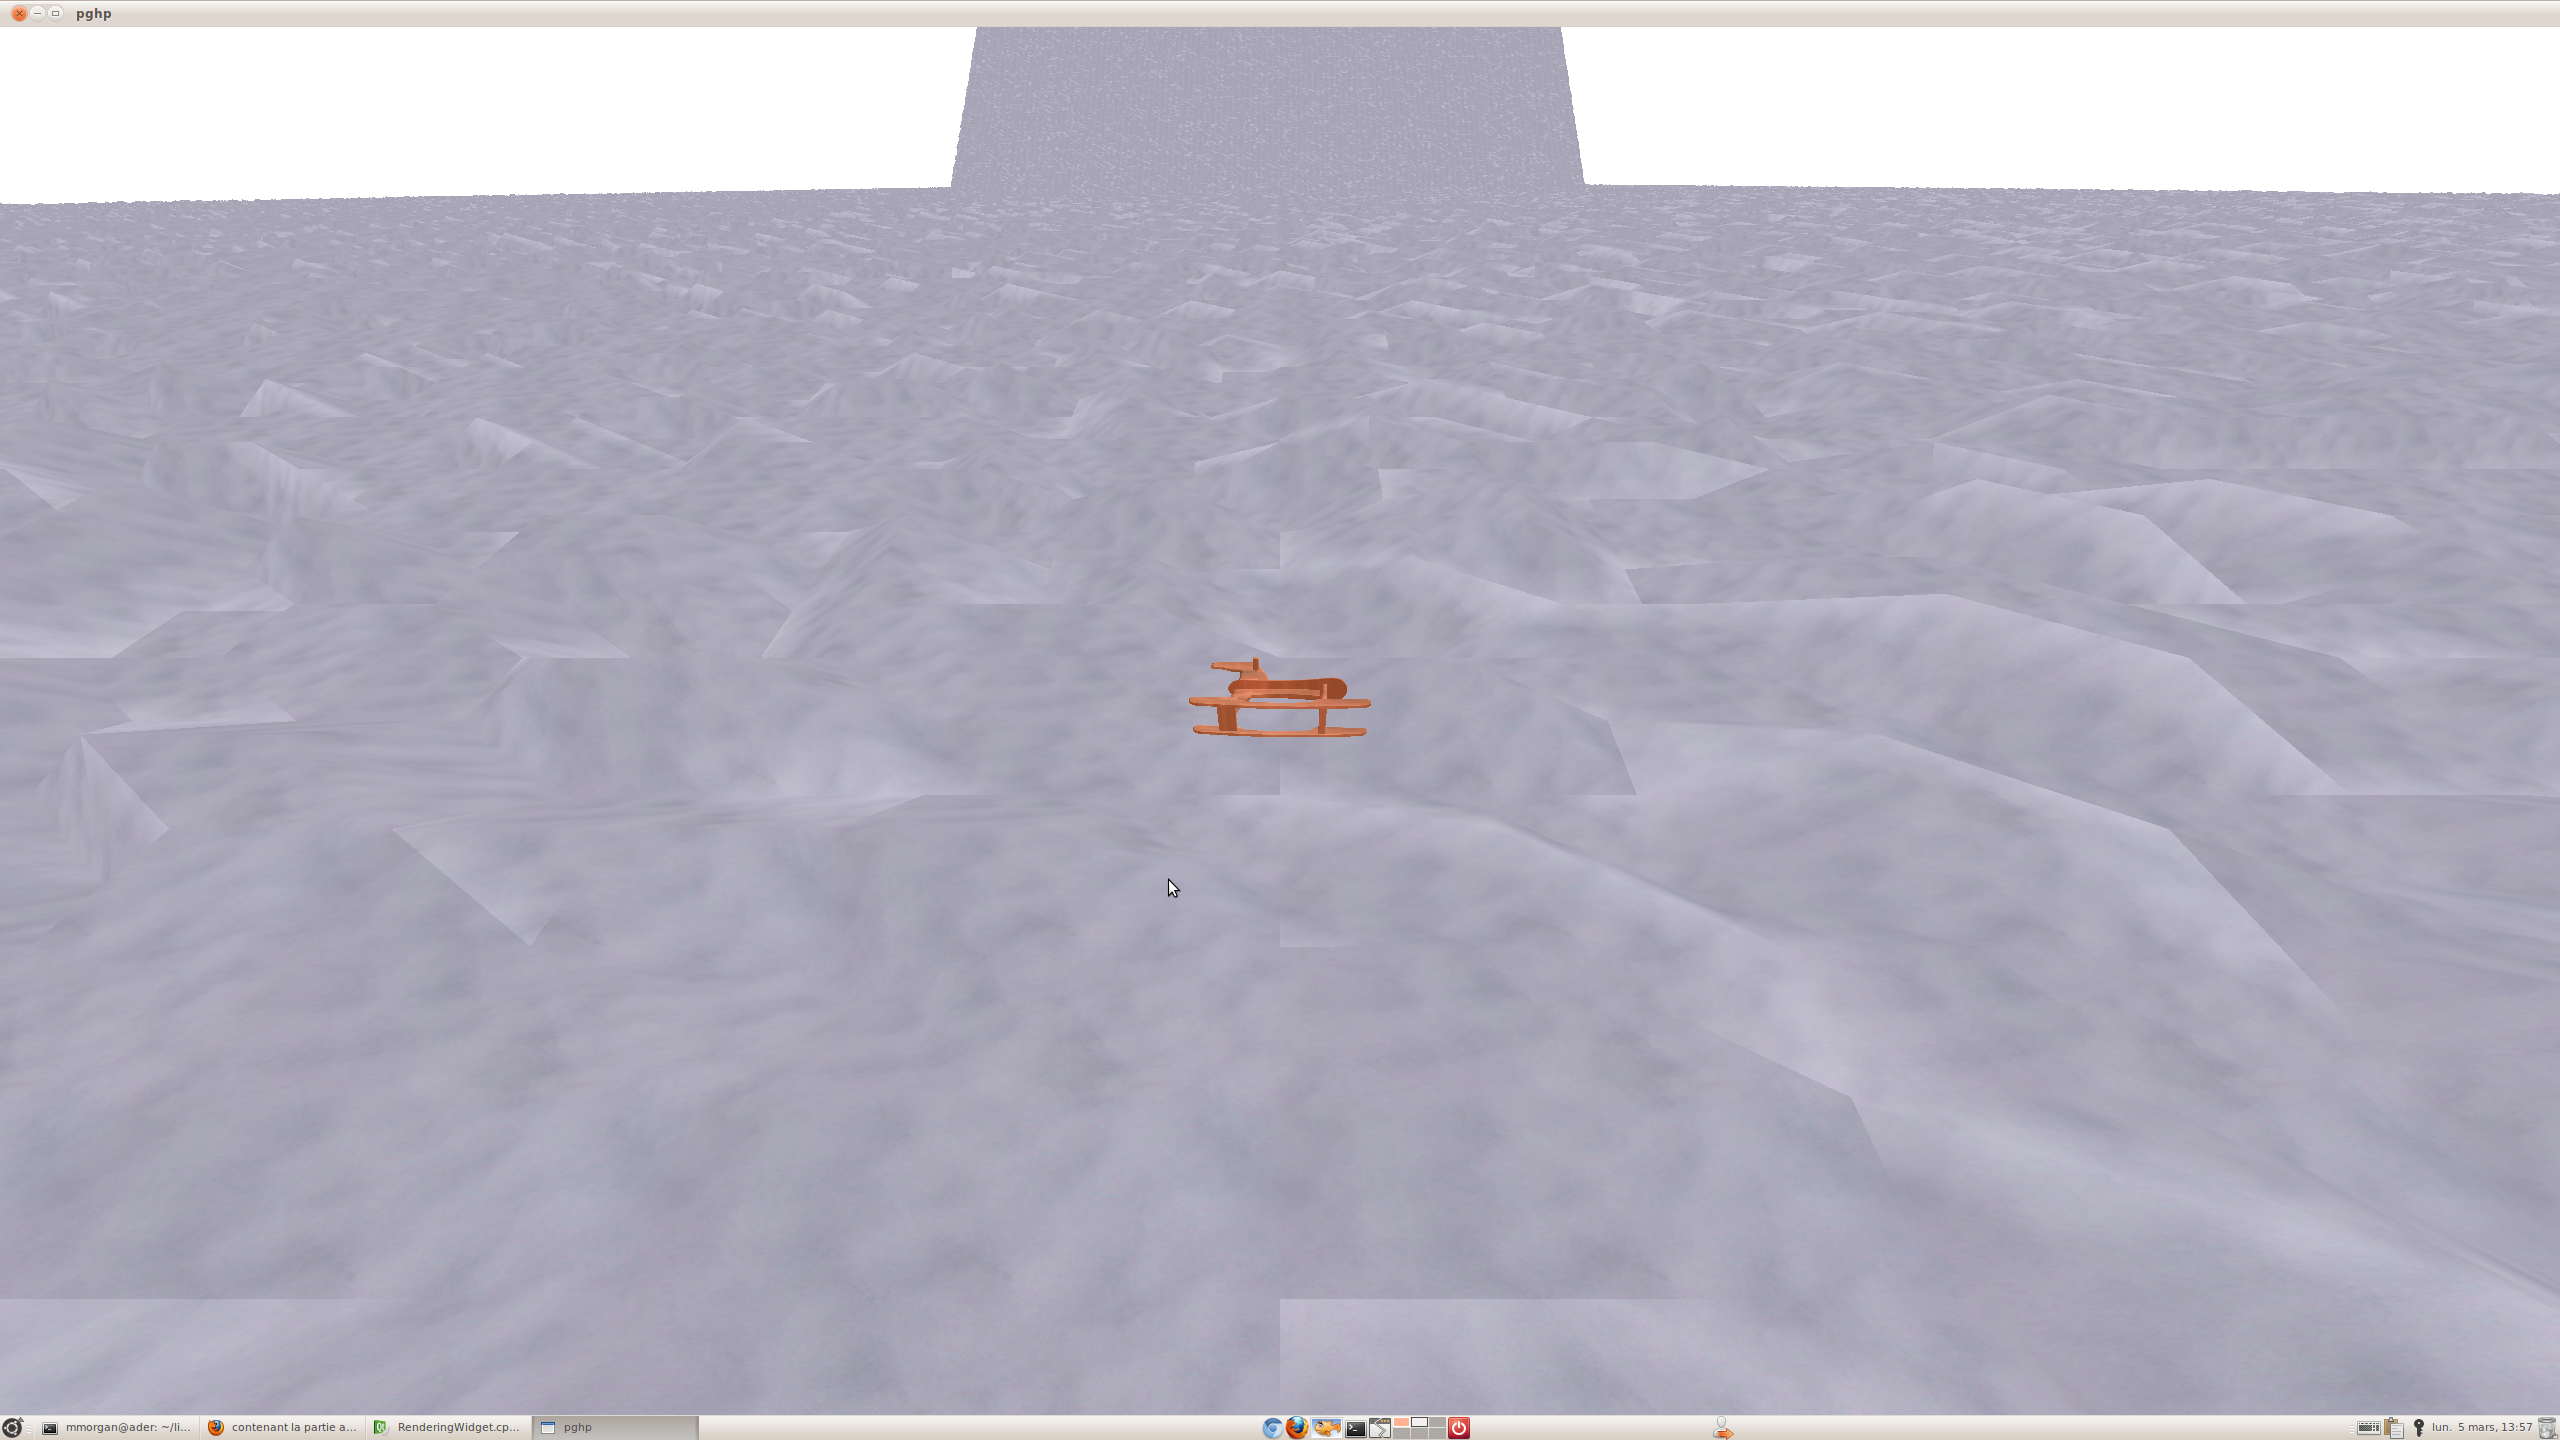
\includegraphics[scale=0.2]{../../../../../../../../net/cremi/aledupou/Desktop/1.png}
\end{figure}

\begin{figure}[hbtp]
\caption{Mode fil de fer}
\centering
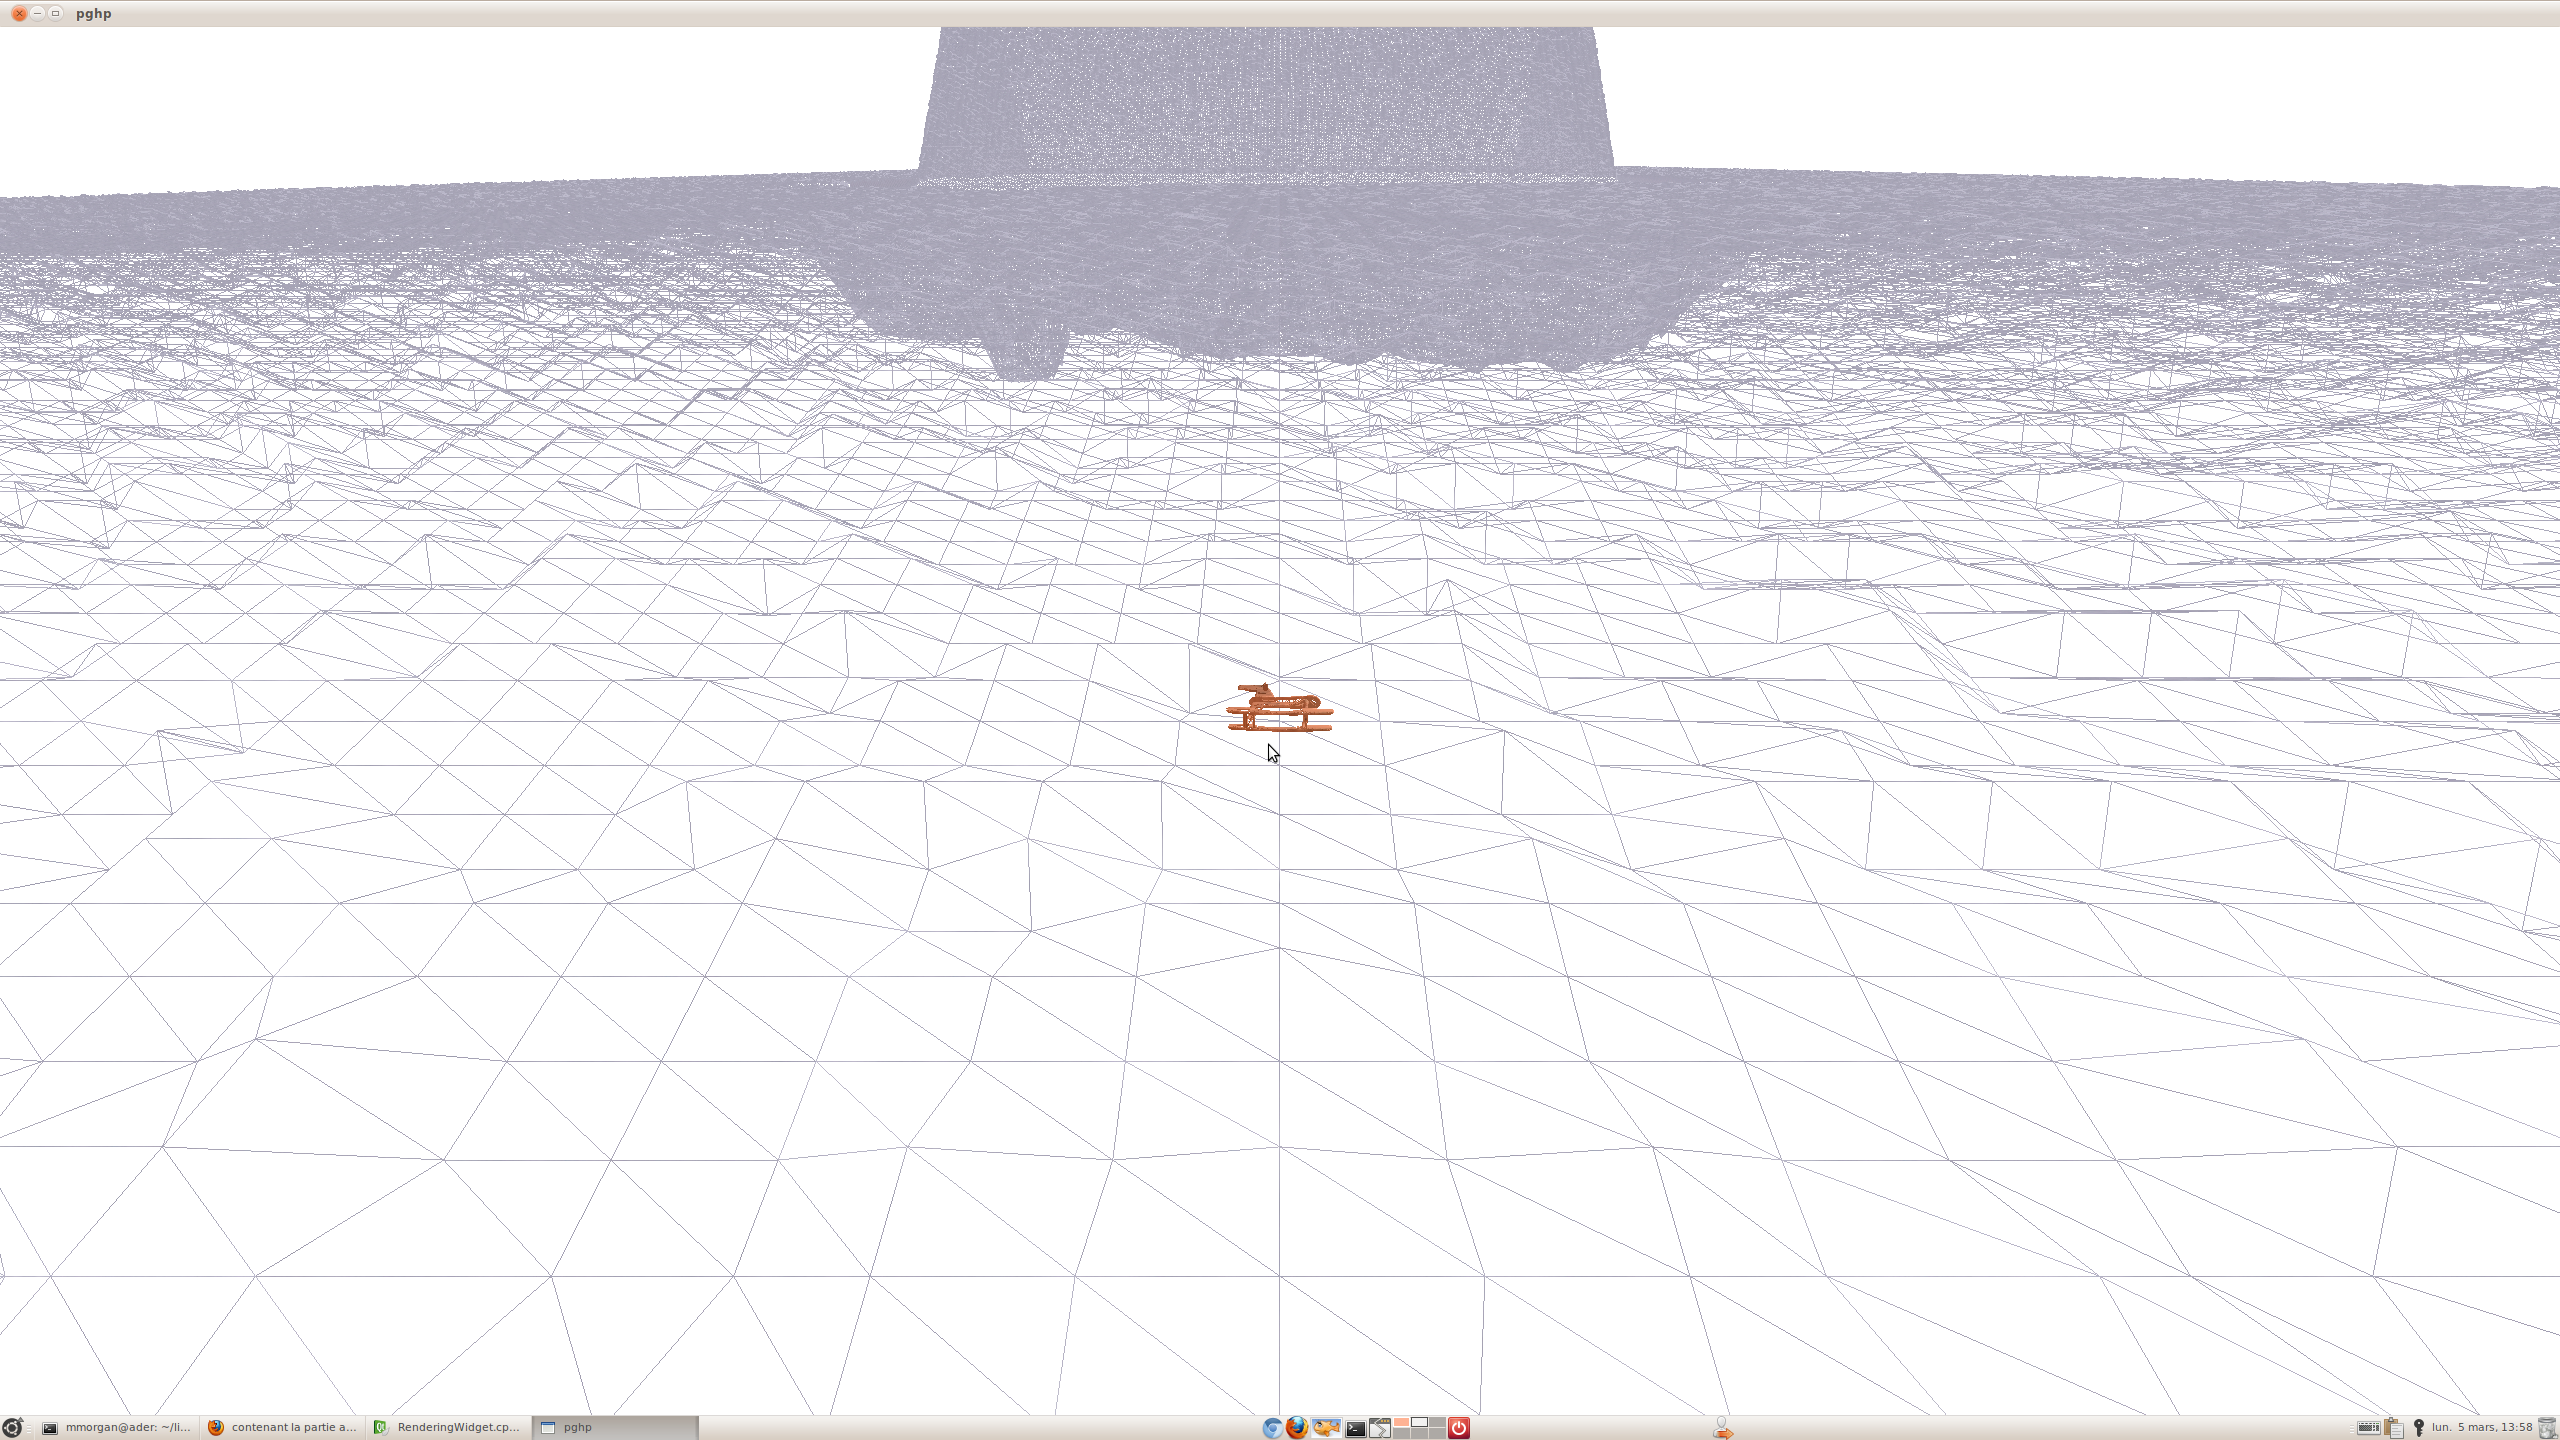
\includegraphics[scale=0.2]{../../../../../../../../net/cremi/aledupou/Desktop/2.png}
\end{figure}

\begin{figure}[hbtp]
\caption{Camera : vue plongeante}
\centering
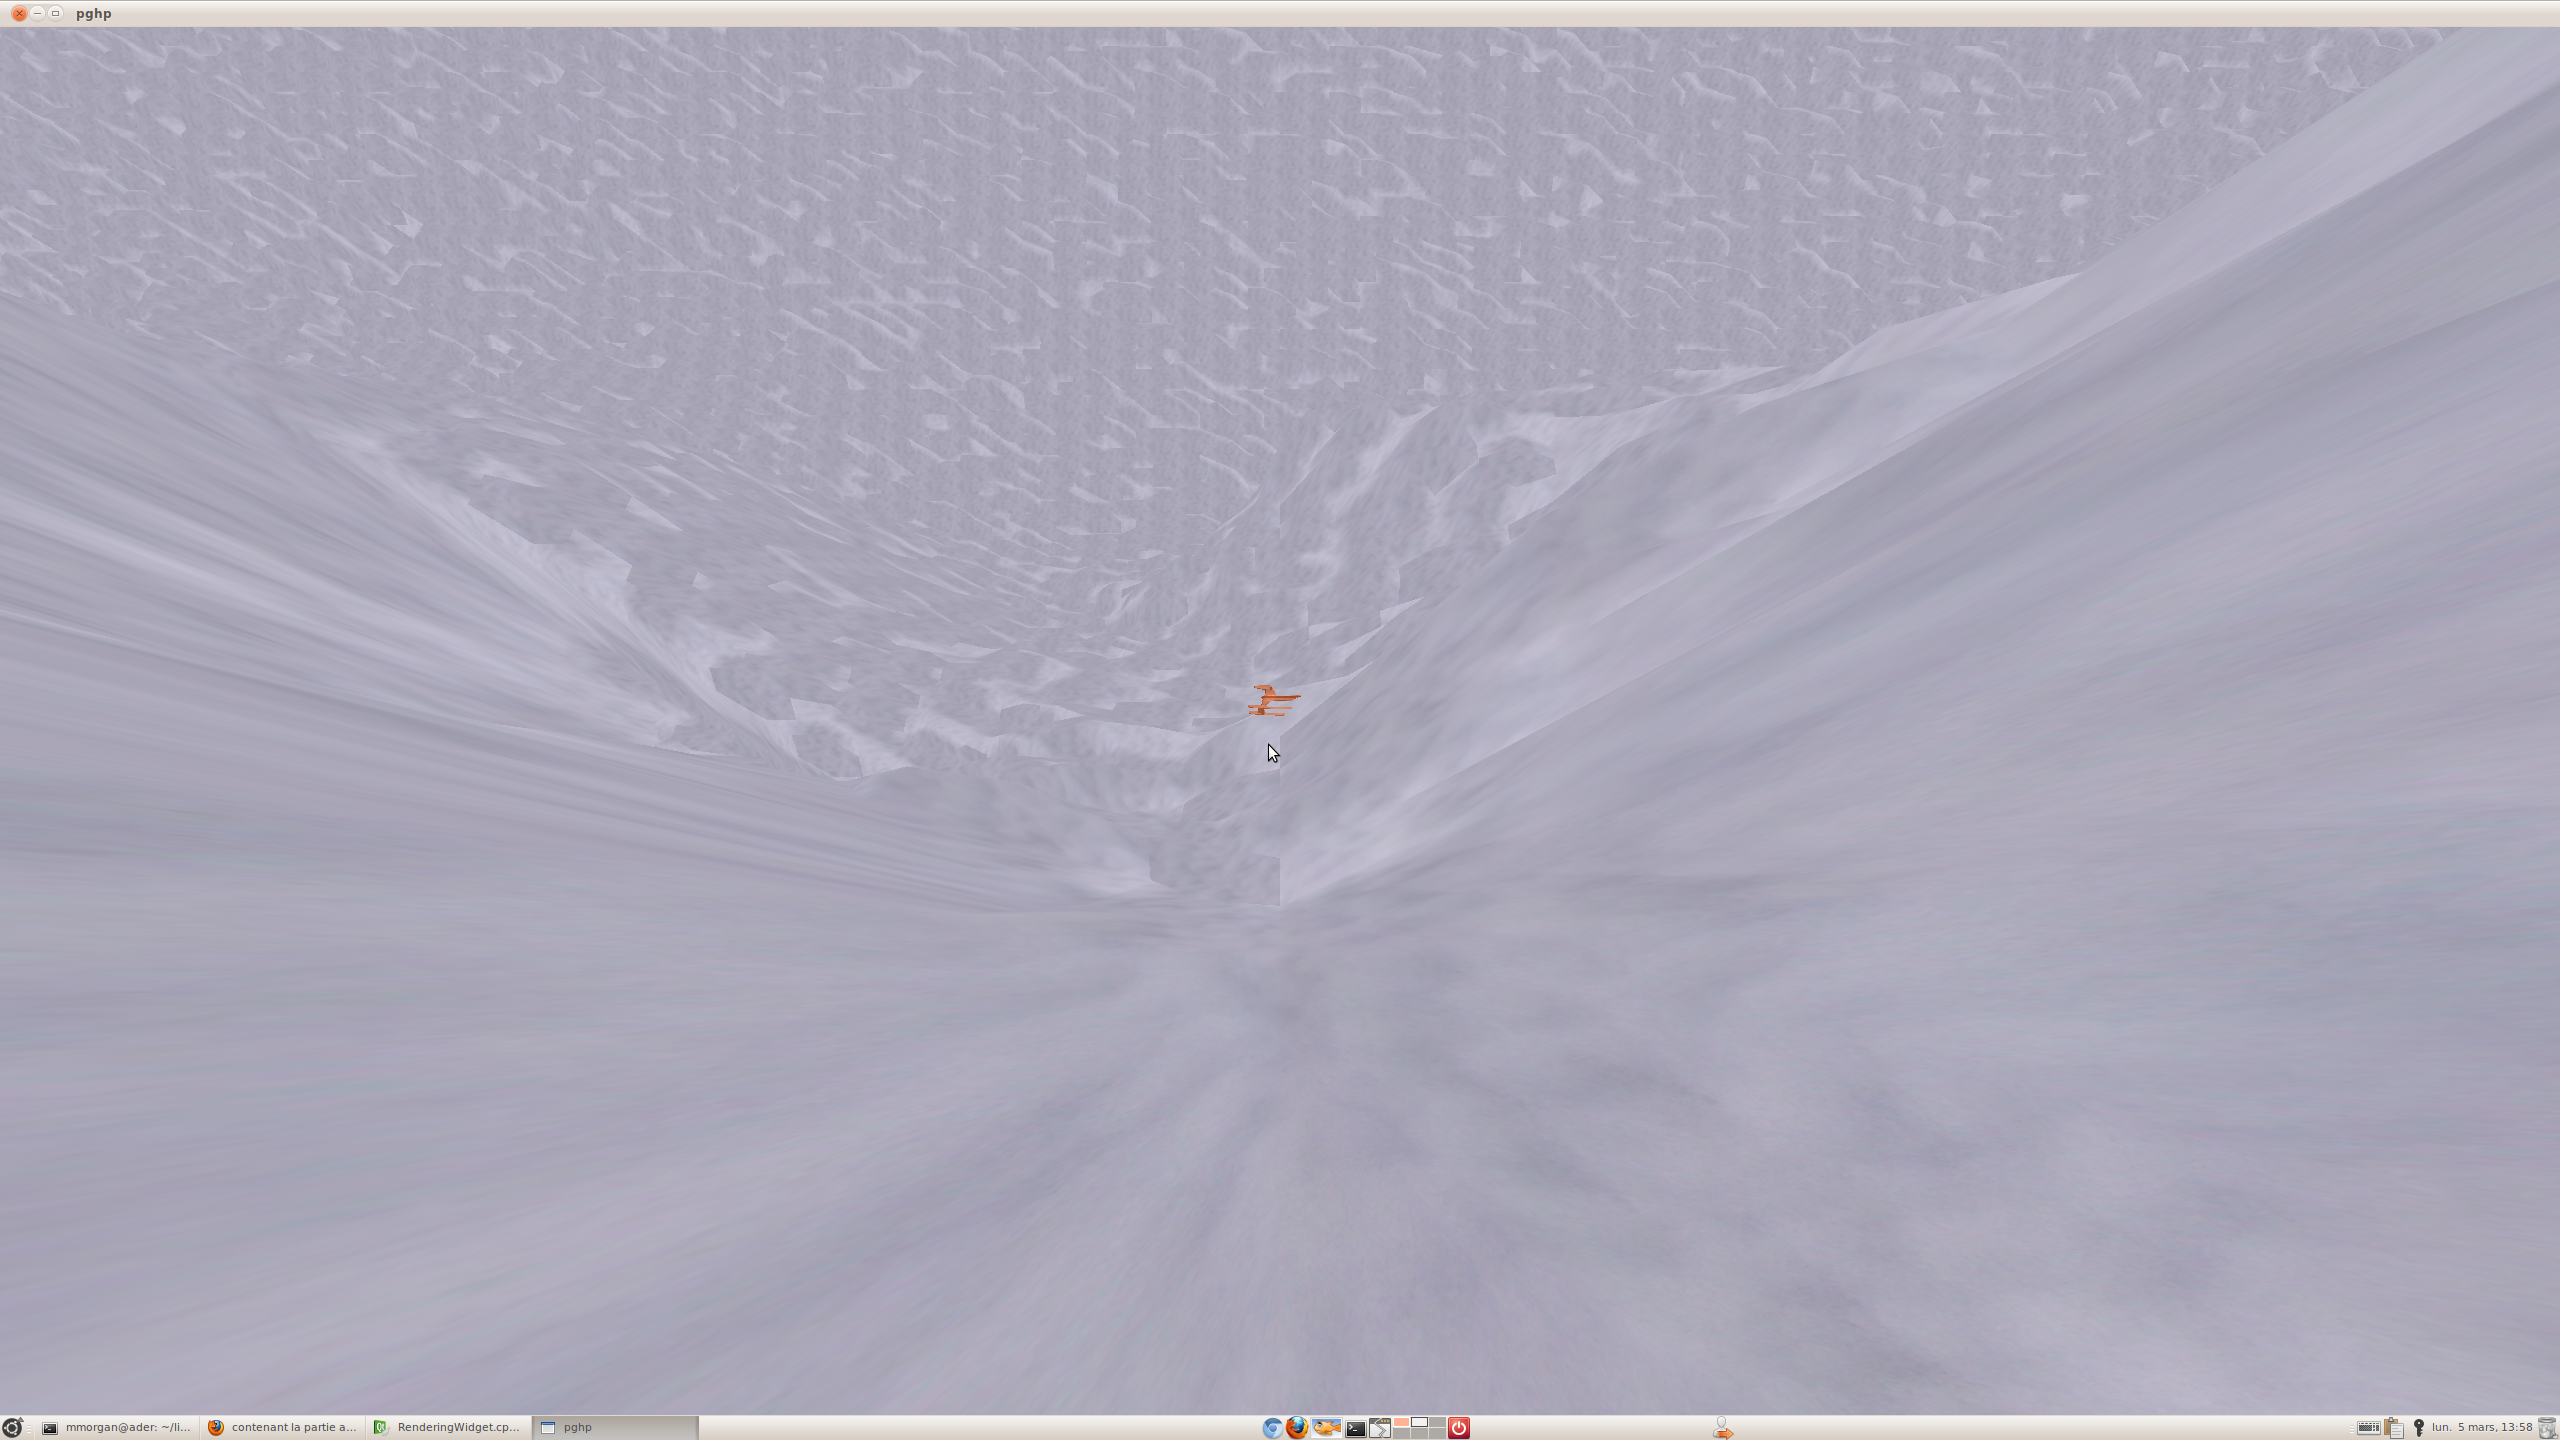
\includegraphics[scale=0.2]{../../../../../../../../net/cremi/aledupou/Desktop/3.png}
\end{figure}

\begin{figure}[hbtp]
\caption{Camera : vue plongeante en mode fil de fer}
\centering
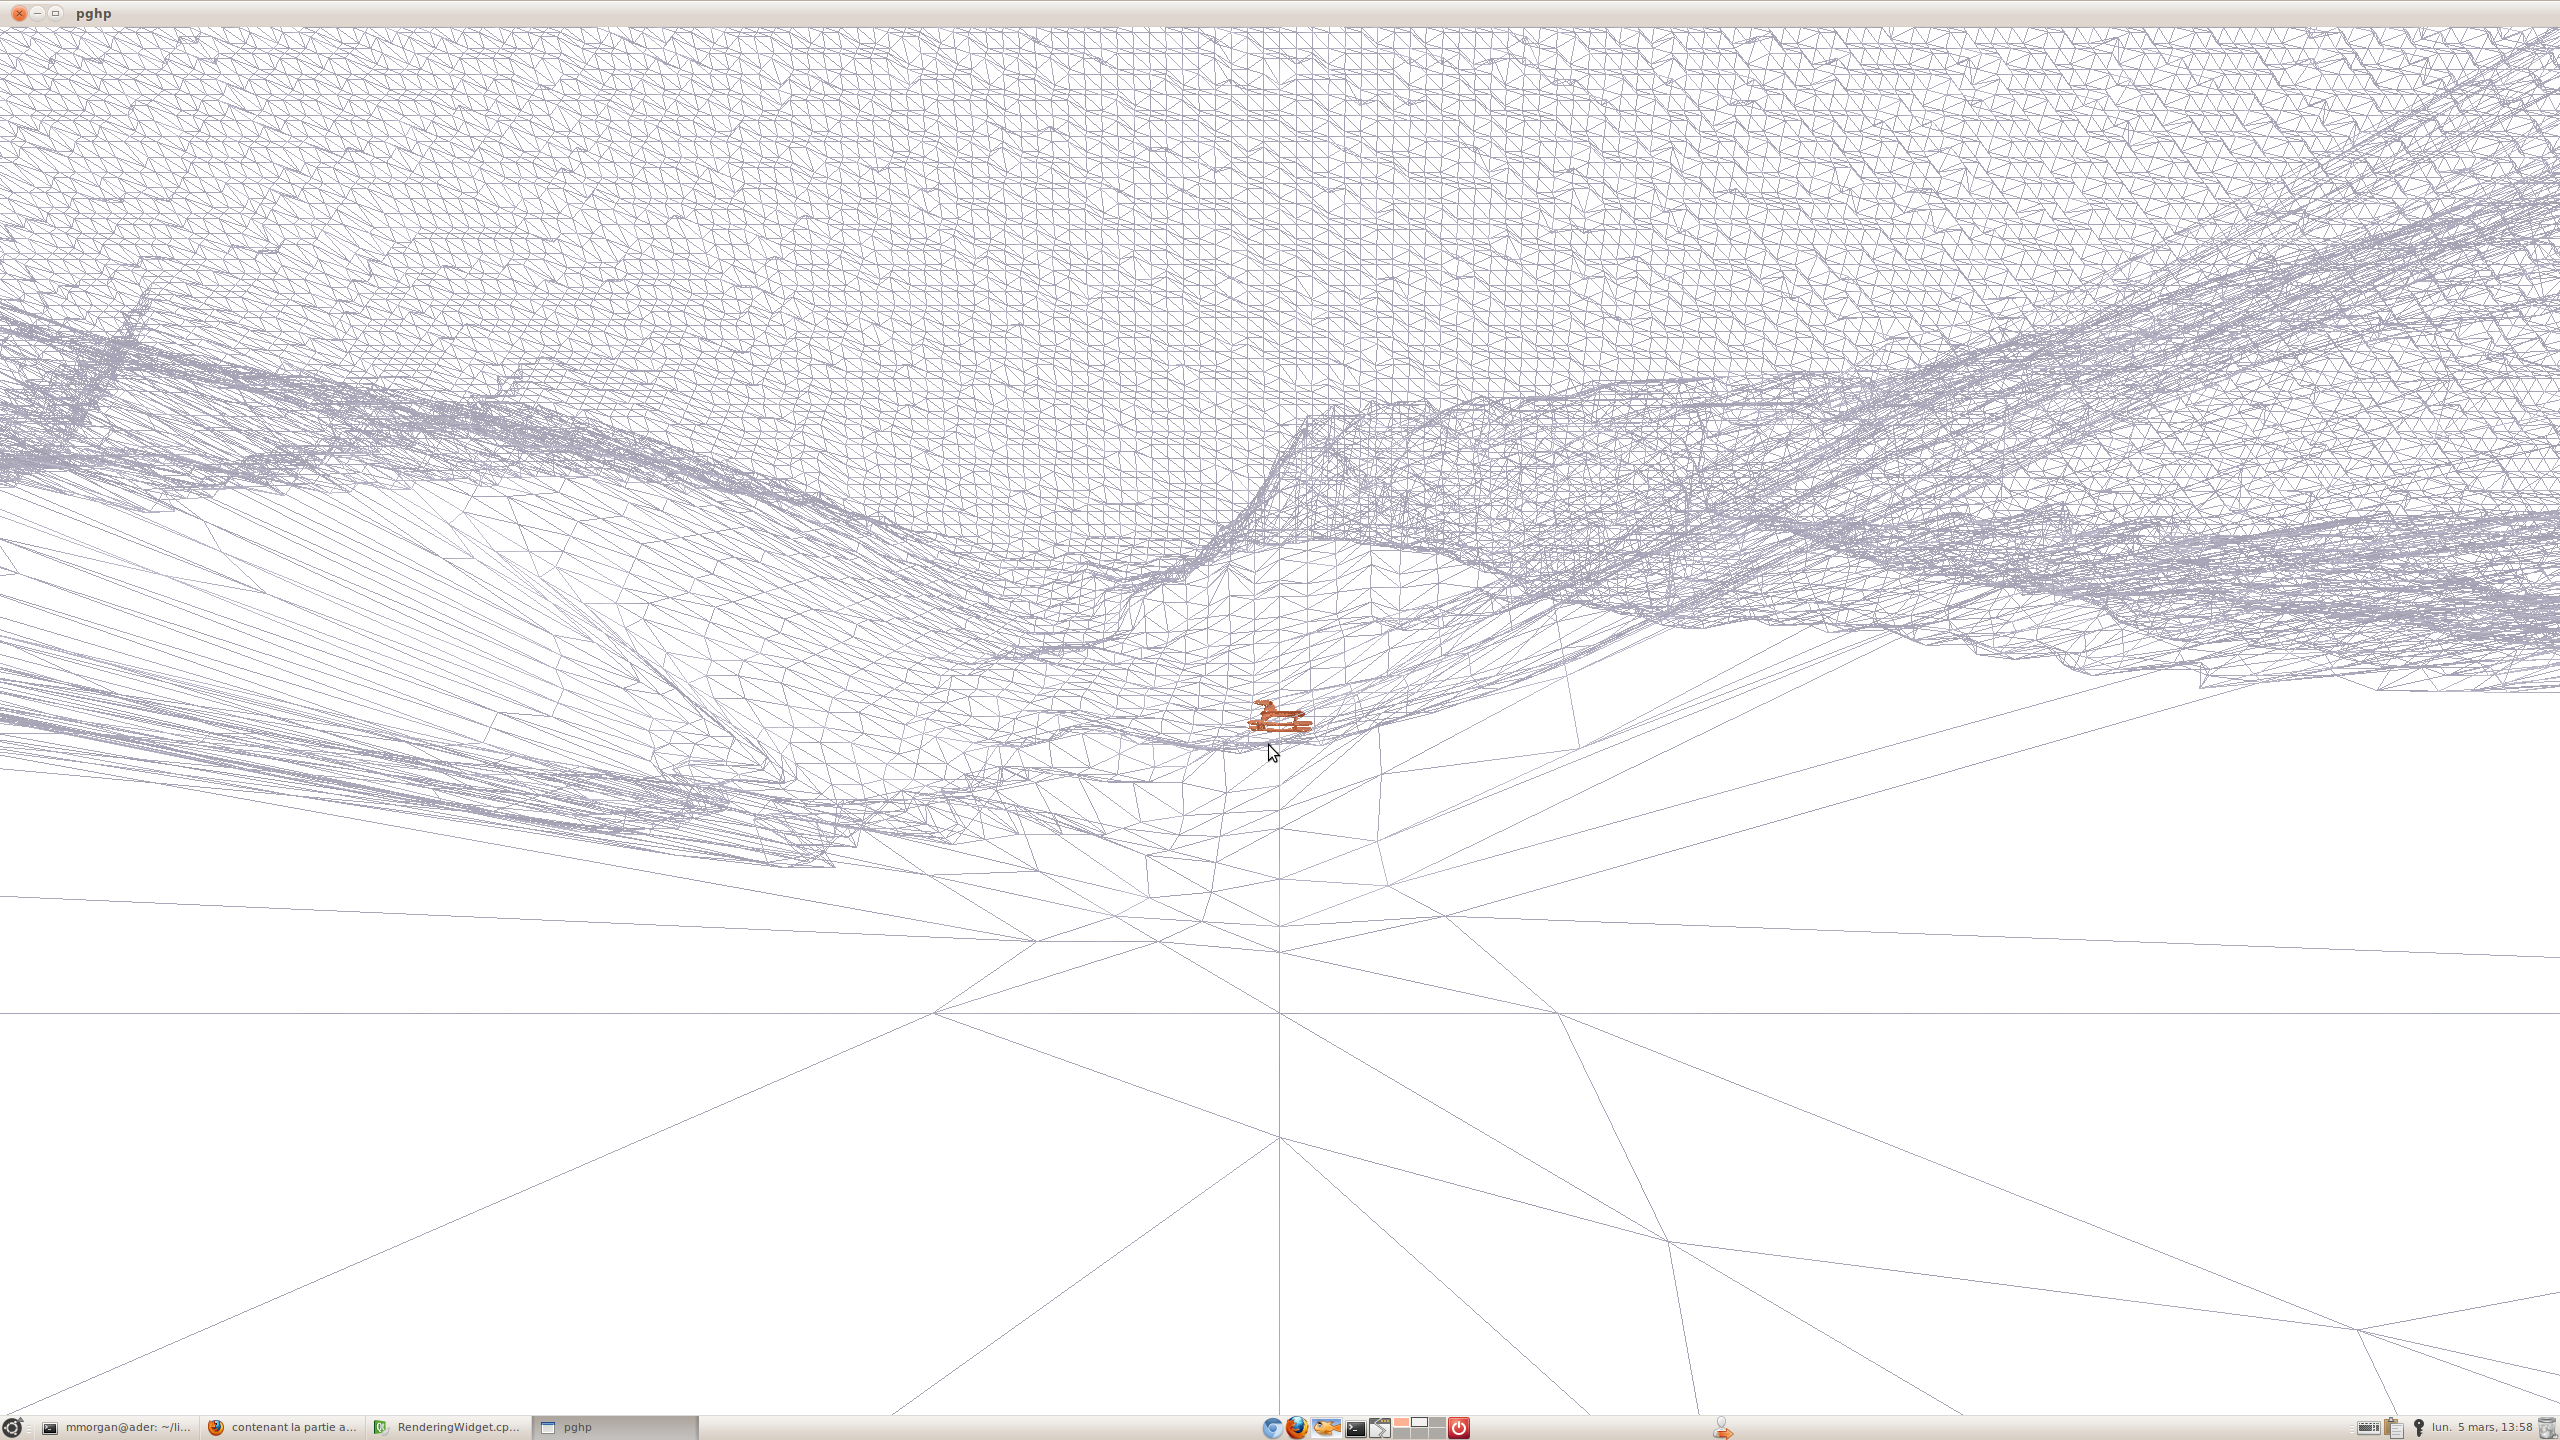
\includegraphics[scale=0.2]{../../../../../../../../net/cremi/aledupou/Desktop/4.png}
\end{figure}



\end{document}